\documentclass[a4paper, 12pt]{report}

\input{preamble}
\pgfplotsset{compat=1.18}

\title{
	{\Huge Mathématiques pour lycéen (niveau seconde)} \\ 
	{\Large Année 2025-2026}
}

\author{\huge{Benjamin Clamme}}
\date{\today}

\begin{document}

\maketitle

Ce cours est librement inspiré de l'ouvrage ``Mathématiques en classe de Seconde, Problèmes et solutions'' par Matthieu Häberle (librement disponible ici : \url{https://github.com/Mattuuuuh/Maths-2nde}). \\

Le cours présente toutes les définitions, propositions et théorèmes qu'un élève de seconde générale doit connaître (et parfois un peu plus).  \\

Si vous trouvez dans ce livre une erreur, un point qui vous semble améliorable ou si, plus largement, vous souhaitez me contacter, mon adresse mail est : benjamin.clamme@ac-clermont.fr.
\newpage

\chapter{Ensembles de nombres}

\section{Prérequis}

\begin{nota}
On appelle ``ensemble'' une collection non ordonnée d'élements quelconques (par exemple des nombres). On note les ensembles avec des accolades et des points-virgules entre les éléments, par exemple :
\[ E = \{ 1 ; 25 ; 3 ; 4 \}. \]
Un ensemble peut éventuellement contenir un nombre infini d'éléments, on pourra alors noter cet ensemble en sous-entendant une partie des éléments, par exemple :
\[ E = \{1 ; 3 ; 5 ; 7 ; \dots \}, \]
ou en exprimant une condition formelle d'appartenance à l'ensemble, par exemple 
\[ E = \{ \text{nombres entiers impairs} \}. \]
On utilisera le symbole ``$\in$'' pour dénoter l'appartenance d'un élément à un ensemble, par exemple :
\[ x \in E \]
signifie que $x$ appartient à $E$ (on dira aussi ``$x$ est un élément de $E$'' ou ``$x$ est dans $E$''). \\
On utilisera le symbole ``$\subset$'' pour dénoter l'inclusion d'un ensemble dans un autre, par exemple :
\[ F \subset E \]
signifie que tous les éléments de $F$ sont aussi des éléménts de $E$, on dit alors que \textbf{$F$ est inclus dans $E$}. On notera au passage que 
\[ (F \subset E) \text{ si, et seulement si, } (x \in F \Rightarrow x \in E). \] 
\end{nota}

\section{Les nombre entiers}

Lorsqu'on évoque ``un nombre'', sans plus de précision, on pense habituellement aux nombres entiers. On prendra garde de distinguer les entiers naturels (les entiers \textbf{positifs}) des entiers relatifs (positifs \textbf{ou négatifs}).

\begin{defn}[Nombres entiers]
L'ensemble des entiers naturels, dénoté par $\N$, est l'ensemble des entiers positifs 
\[ \N = \{0 ; 1; 2 ; \dots \}. \]
L'ensembles des entiers relatifs, dénoté par $\Z$, est l'ensemble de tous les entiers 
\[ \Z = \{ \dots ; -3 ; -2; -1 ; 0 ; 1 ; 2 ; 3 ; \dots \}. \]
\end{defn}

\begin{prop}
L'ensemble des entiers naturels est inclus dans l'ensemble des entiers relatifs : $\N \subset \Z$.
\end{prop}

\begin{rmq}
Les entiers naturels sont simplement des entiers relatifs de signe positif.
\end{rmq}

\section{Développement décimal et nombres décimaux}

Les nombres décimaux sont ceux ``que l'on peut écrire sur un morceau de papier (éventuellement très grand)''. La définition formelle de cet ensemble est donnée ci-dessous.

\begin{defn}[Développement décimal]
Le développement décimal d'un nombre correspond à son écriture en base $10$, y compris les puissances négatives de $10$.
\end{defn}

\begin{ex}
Le développement décimal de $\frac{1}{4}$ correspond à $0,25$ (ou encore $0 \times 10^0 + 2 \times 10^{-1} + 5 \times 10^{-2}$).
\end{ex}

\begin{defn}[Nombres décimaux]
Un nombre est dit décimal si son développement décimal est \textbf{fini}. On note $\Dom$ l'ensemble des nombres décimaux.
\end{defn}

\begin{ex}
Le nombre $\frac{1}{4}$ est bien un nombre décimal, car son développement décimal comporte exactement trois chiffres (dont deux après la virgule).
\end{ex}

\begin{thm}[Caractérisation de $\Dom$]
\[ \Dom = \left \{ \frac{a}{10^n} \text{ tel que } a \in \Z, n \in \N \right \} . \]
\end{thm}

\begin{proof}
Cette démonstration utilise un format de preuve classique (par double inclusion), il est donc particulièrement intéressant de bien la comprendre. On va poser $E = \left \{ \frac{a}{10^n} \text{ tel que } a \in \Z, n \in \N \right \}$ et on va montrer que $E = \Dom$. Pour ce faire, on va d'abord montrer que $\Dom \subset E$ puis que $E \subset \Dom$. Les deux ensembles étant mutuellement inclus l'un dans l'autre, ils sont nécessairement égaux (faites un dessin !). \\

\underline{Démonstration de $\Dom \subset E$ : } soit $x$ un élément de $\Dom$, comme $x$ a un développement décimal fini, on peut ``compter'' le nombre de ses chiffres après la virgule. En notant $n$ ce nombre, on a $10^n \cdot x \in \Z$ et, par suite, $x = \frac{a}{10^n}$ avec $a \in \Z$, soit $x \in E$. Ceci étant vrai pour tout élément de $\Dom$, on en déduit que $\Dom \subset E$. \\

\underline{Démonstration de $E \subset \Dom$ : } soit $x$ un élément de $E$, on écrit $x =  \frac{a}{10^n}$ avec $a \in \Z$ et $n \in \N$. Comme $a$ est un entier, son développement décimal est fini et la division par $10^n$ ne fait que ``déplacer la virgule'' (ce qui ajoute au plus $n$ zéros au développement décimal de $a$), donc $x \in \Dom$. Ceci étant vrai pour tout élément de $E$, on en déduit que $E \subset \Dom$. \\
\end{proof}

\begin{coro}
L'ensemble des entiers relatifs est inclus dans l'ensemble des nombres décimaux
\[ \Z \subset \Dom. \]
\end{coro}

\begin{proof}
Il suffit de remarquer que si $a \in \Z$ alors $a = \frac{a}{10^0} \in \Dom$. Donc $\Z \subset \Dom$.
\end{proof}

\begin{prop}
Le nombre $\frac{1}{3}$ \textbf{n'est pas} un nombre décimal
\end{prop}

\begin{proof}
Pour démontrer ce résultat, on va réaliser une \textbf{démonstration par l'absurde}, 
c'est-à-dire supposer que l'assertion est vraie et montrer que cela est absurde. 
Si $\frac{1}{3}$ est décimal, alors il existe $a \in \Z$ et $n \in \N$ tels que :
\[ \frac{1}{3} = \frac{a}{10^n} \Rightarrow 10^n=3a . \]
Autrement dit, $10^n$ est un multiple de $3$. Or $10^n-1 \in \{0, 9, 99, 999, \dots \}$ donc $10^n-1$ est un multiple de $3$. 
Ainsi $10^n$ ne peut pas être un multiple de trois, on a donc une contradiction.
\end{proof}

\begin{rmq}
On aurait aussi simplement affirmer que $\frac{1}{3} = 0,333 \dots$ et donc que $\frac{1}{3}$ n'est pas décimal car son \textbf{unique}
développement décimal n'est pas fini. Il reste cependant à prouver que le développement décimal de $\frac{1}{3}$ 
\textbf{est en effet unique}. 
Par exemple, le nombre $1$ admet deux développements décimaux, $1$ et $0,999 \dots$ 
(ce dernier étant appelé développement décimal impropre). 
C'est pour esquiver ces subtilités que la preuve par l'absurde ci-dessus est proposée.
\end{rmq}

\section{Les nombres rationnels}

Les nombres rationnels sont ceux ``que l'on peut mettre sous forme de fraction''. La définition formelle de cette ensemble est donnée ci-dessous.

\begin{defn}[Nombres rationnels]
Soient $a,b \in \Z$ deux entiers relatifs, avec $b$ non nul. Le nombre rationnel $\frac{a}{b}$ est l'unique nombre tel que 
\[ \frac{a}{b} \times b = a. \]
L'ensemble des nombres rationnels est noté 
\[ \Q = \left \{ \frac{a}{b} \text{ tels que } a, b \in \Z, b \neq 0 \right \}. \]
\end{defn}

\begin{ex}
Le nombre rationnel $\frac{1}{2}$ est l’unique nombre vérifiant $\frac{1}{2} \times 2 = 1$.
\end{ex}

\begin{prop}
L'ensemble des nombres décimaux est inclus dans l'ensemble des nombres rationnels :
\[ \Dom \subset \Q. \]
\end{prop}

\begin{proof}
Soit $x \in \Dom$, il existe $a \in \Z$ et $n \in \N$ tels que $x = \frac{a}{10^n}$. Or $10^n \in \Z$ et $10^n \neq 0$ ($10^0 = 1, 10^1 = 10, \dots$) donc, en posant $b=10^n$ on a bien $x=\frac{a}{b}$ avec $a, b \in \Z$ et $b \neq 0$.
\end{proof}

\begin{thm}
Soient $a, b, c ,d \in \Z$ avec $b$ et $d$ non nuls. On a 
\[ \frac{a}{b} \cdot \frac{c}{d}  = \frac{ac}{bd} \in \Q \qquad \text{et} \qquad \frac{a}{b} + \frac{c}{d} = \frac{ad + bc}{bd} \in \Q. \]
\end{thm}

\begin{proof}
Voir TD n°2.
\end{proof}

\begin{coro}
Soient $a, b , c \in \Z$ avec $c$ non nul, on a
\[ \frac{a}{b} = \frac{ac}{bc} \]
\end{coro}

\begin{proof}
Démontrons d'abord que $\frac{c}{c} = 1$. En utilisant la définition, $\frac{c}{c}$ est l'unique nombre tel que $\frac{c}{c} \cdot c = c$, 
or $1 \cdot c = c$, on en déduit (par unicité) que $\frac{c}{c} = 1$. \\
On utilise maintenant le théorème, $\frac{ac}{bc} = \frac{a}{b} \cdot \frac{c}{c} = \frac{a}{b}$.
\end{proof}

\begin{rmq}
Ce corollaire justifie la définition suivante.
\end{rmq}

\begin{defn}
On dit qu'une fraction est irréductible si elle est sous la forme $\dfrac{a}{b}$ avec $a$ et $b$ premiers entre eux. Autrement dit, \textbf{on ne peut plus simplifier la fraction}.
\end{defn}

\begin{rmq}
Un nombre rationnel admet plusieurs écritures (par exemple $\dfrac13 = \dfrac26 = \dfrac4{12} \dots$. Cependant, il existe une écriture plus simple que les autres, c'est celle sous forme d'une fraction irréductible. Dans la suite de ce paragraphe, on va voir qu'il existe une autre façon de caractériser les éléments de $\Q$.
\end{rmq}

\begin{defn}
On dit que le développement décimal d’un nombre est éventuellement périodique dès qu’il se répète à partir d’un certain point.
\end{defn}

\begin{ex}
\label{ex:dev-dec}
\begin{enumerate}
\item Le développement décimal du nombre $\dfrac13$ est périodique, il se répète dès le premier chiffre après la virgule $\left ( \dfrac13 = 0,3333 \dots \right )$ et la période est de longueur $1$ (elle est constitué d'un seul chiffre, à savoir $3$).
\item Le développement décimal du nombre $\dfrac17$ est aussi périodique. Pour le démontrer on utilise l'algorithme suivant :
\begin{enumerate}
\item On effectue la division euclidienne de 1 par 7, soit $1 = 7 \times 0 + 1$.
\item On prend le reste de l'étape précédente et on le multiplie par 10, on effectue la division euclidienne de ce nombre par 7 soit
$10 = 7 \times 1 + 3$.
\item On itère l'étape précédente avec le reste obtenu à cette même étape.
\end{enumerate}
\end{enumerate}
Les restes possibles appartenant à l'ensemble $\{0, 1, 2, 3, 4, 5, 6 \}$ et, le reste obtenu à l'étape $n+1$ étant déterminé par celui obtenu à l'étape $n$, on obtient éventuellement une période dans le développement décimal.
\end{ex}

\begin{thm}[Caractérisation décimale de $\Q$]
Un nombre est rationnel si, et seulement si, son développement décimal est périodique.
\end{thm}

\begin{proof}
Pour démontrer que tout nombre rationnel admet un développement décimal périodique, on peut employer l'algorithme utilisé à l'exemple $\ref{ex:dev-dec}$. Lorsqu'on effectue des divisions euclidiennes successives, il y a un nombre fini de restes possibles et le reste obtenu à l'étape $n+1$ est déterminé par celui obtenu à l'étape $n$, le développement décimal est donc éventuellement périodique.

Réciproquement, prenons $x$ un nombre admettant un développement décimal périodique. Supposons que le développement décimal de $x$ soit périodique à partir du $n$ième chiffre après la virgule et que la période soit de longueur $p$ (i.e. qu'elle comporte $p$ chiffres). Alors $10^{n+p-1} x - 10^{n-1} x = (10^{n+p-1}  - 10^{n-1}) x$ est un entier soit 
\[ (10^{n+p-1}  - 10^{n-1}) x = d, \text{ avec } d \in \Z \Rightarrow x = \frac{d}{(10^{n+p-1}  - 10^{n-1})} \in \Q. \]
\end{proof}

Jusqu'ici, nous avons défini quatre ensembles de nombres (les entiers naturels, puis relatifs, les nombres décimaux et les nombres rationnels) tels que :
\[ \N \subset \Z \subset \Dom \subset \Q. \]
On peut légitimement se demander si ces quatre ensembles ne sont pas suffisant pour décrire \textbf{tous} les nombres que l'on peut imaginer.

\begin{lem}
Soit $a \in \Z$ un nombre entier ; $a^2$ est pair si et seulement si $a$ est pair.
\end{lem}

\begin{proof}
Supposons que $a^2$ est pair, alors $a^2-1$ est impair. Or $a^2-1=(a-1)(a+1)$. Si $a$ est impair, alors $a-1$ et $a+1$ sont pairs ce qui est impossible (puisque $a^2-1$ est impair !) donc $a$ est pair. La réciproque (si $a$ est pair alors $a^2$ est pair) se démontre très facilement (faites le en exercice).
\end{proof}

\begin{prop}
Il existe un nombre non-rationnel.
\end{prop}

\begin{proof}
On considère le nombre $\sqrt{2}$, on suppose que $\sqrt{2} \in \Q$, il existe donc $a, b \in \Z$ tels que $\sqrt{2}=\frac{a}{b}$. On suppose de plus que la fraction $\frac{a}{b}$ est sous forme irréductible. On remarque que :
\[ \sqrt{2} b = a \equi 2 b^2 = a^2 \qquad (\ast) \]
donc $a^2$ est pair et, d'après le lemme, $a$ est pair. Il existe donc $n \in \Z$ tel que $a=2n$. En substituant dans $(\ast)$ on obtient 
\[ 2 b^2 = 4 n^2 \equi b^2 = 2 n^2 \]
donc $b^2$ est pair et, toujours d'après le lemme, $b$ est pair. Il existe donc $m \in \Z$ tel que $b=2m$. Finalement, on peut écrire 
\[ \sqrt{2} = \frac{a}{b} = \frac{2n}{2m} \]
autrement dit, la fraction $\frac{a}{b}$ est réductible (on peut diviser par 2 !) ce qui est contradictoire. Donc $\sqrt{2}$ n'est pas rationnel.
\end{proof}

\begin{rmq}
Les nombres non rationnels sont appelés ``nombres irationnels''. $\pi$ est aussi un nombre irrationnel.
\end{rmq}

\section{Les nombres réels}

\begin{defn}
On appelle \textbf{nombres réels} l'ensemble de tous les nombres et on le note $\R$. Cet ensemble est infini et \textbf{continu}.
\end{defn}

La continuité des réels signifie que, si l'on se visualise l'ensemble des réels comme une droite infinie, alors les nombres réels occupe toute la droite, sans laisser de trou.

\begin{center}
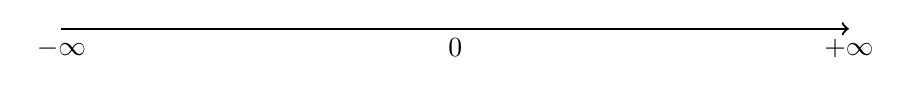
\begin{tikzpicture}[scale=1]
\draw[->, thick] (-5,0) node[below] {$-\infty$} -- (0,0) node[below] {$0$} -- (5,0) node[below] {$+\infty$};
\end{tikzpicture}
\end{center}

De plus, si on prend deux points distincts au hasard sur cette droite (par exemple $x$ et $y$ avec $x<y$), alors l'intervalle $[x,y]$ contiendra \textbf{une infinité non dénombrable} de points. On traitera cette notion plus avant dans un prochaine chapitre.

\begin{rmq}
On a les inclusions suivantes :
\[ \N \subset \Z \subset \Dom \subset \Q \subset \R \]
\end{rmq}

\begin{thm}
Soit $x$ un nombre réel et $n$ un entier naturel. 
Alors il existe deux nombres décimaux $r$ et $s$ tels que
\[ r \leq x \leq s \qquad \text{et} \qquad s-r \leq 10^{-n} \]
\end{thm}

\begin{proof}
On considère le nombre $10^n x$, qui est obtenu en décalant $n$ fois la virgule vers la gauche dans $x$. 
On retire tous les chiffres après la virgule dans $10^n x$ et on note $a$ le nombre entier ainsi obtenu, on a
\[ a \leq 10^n x \leq a+1 \]
On pose ensuite $r = \frac{a}{10^n}$ et $s =\frac{a+1}{10^n}$, on a bien
\[ 10^n r \leq 10^n x \leq 10^n s \Rightarrow r \leq x \leq s . \]
De plus $s-r = \frac{1}{10^n} = 10^{-n}$. 
\end{proof}

\begin{rmq}
La suite d'inégalité $r \leq x \leq s$ est appelé un encadrement de $x$ et la différence $s-r$ est appelée l'amplitude de l'encadrement. 
La proposition précédente affirme que, pour tout réel, il existe un encadrement de $x$ par des nombres décimaux et d'amplitude aussi faible que l'on souhaite.
\end{rmq}

\chapter{Plan cartésien}

Pour un élève placé face à une feuille de papier quadrillé, il semble bien naturel de représenter des figures géométriques 
en s'appuyant sur des lignes perpendiculaires et parallèles et régulièrement espacées. 
Néanmoins, cette idée de ``repérer'' le plan n'est, à notre connaissance, pas si ancienne. 
Elle nous est due à deux penseurs français, René Descartes et Pierre de Fermat, dont les noms sont bien connus des Mathématiciens. \\

Cette idée repose sur l'observation simple que le plan présente deux degrés de liberté, 
autrement dit qu'il est la résultante d'un mouvement selon deux axes (par exemple l'horizontal et la verticale). 
Ainsi, il parait raisonnable d'associer, à chaque point du plan, deux coordonnées indiquant la position du point dans le plan.
Comme de plus, nous avons vu dans le chapitre précédent que l'ensemble des réels peut-être représenté par une droite,
il semble naturel de prendre deux exemplaires de la droite réelle et de les agencer de telle façon à former un repère du plan.

\section{Repère orthonormé}

\begin{defn}[Repère du plan]

Un repère du plan est un système composé de trois points $O, I$ et $J$ déterminant deux droites sécantes
$(OI)$ et $(OJ)$.

	\begin{itemize}
		\item Le point $O$ est appelé l'origine du repère.
		\item La droite $(OI)$ est appelée l'axe des abscisses. La longueur du segement $[OI]$ détermine la graduation 			le long de cet axe.
		\item La droite $(OJ)$ est appelée l'axe des ordonées. La longueur du segement $[OJ]$ détermine la 						graduation le long de cet axe.
		\item La graduation est \textbf{toujours} régulière.
	\end{itemize}
\end{defn}

\begin{ex}
\textit{Un exemple de repère du plan}
\begin{center}
	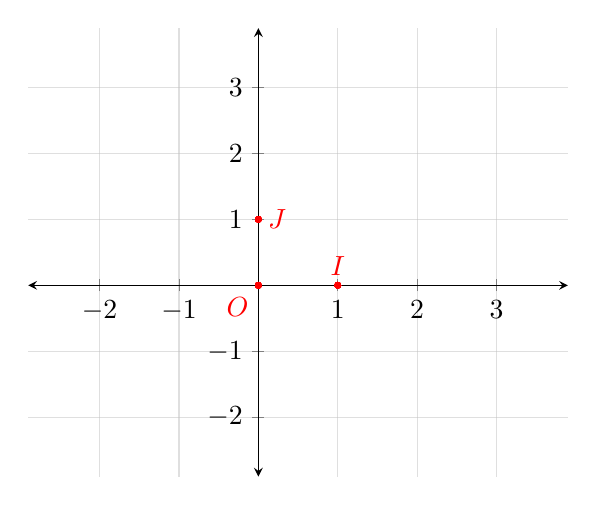
\begin{tikzpicture}[>=stealth, scale=1]
		\begin{axis}[xmin = -2.9, xmax=3.9, xtick={ -3, ..., 5}, ymin=-2.9, ymax=3.9, ytick={-3, ..., 5}, axis x line=middle, axis y 			line=middle, axis line style=<->, xlabel={}, ylabel={}, grid=both, grid style = {opacity=.5}]
		
			\addplot[red, mark=*, mark size = 1] (0,0) node[below=8pt, left] {$O$};
			\addplot[red, mark=*, mark size = 1] (1,0) node[above] {$I$};
			\addplot[red, mark=*, mark size = 1] (0,1) node[right] {$J$};
		\end{axis}
	\end{tikzpicture}
\end{center}
\end{ex}

\begin{defn}[Repère orthonormé]
	Un repère $(O; I, J)$ est
	\begin{enumerate}
		\item \textbf{orthogonal} si ses axes $(OI)$ et $(OJ)$ sont perpendiculaires ;
		\item \textbf{normé} si les segments $[OI]$ et $[OJ]$ sont de même longueur (fixée à $1$) ;
		\item \textbf{orthonormé} s'il est orthogonal et normé.
	\end{enumerate}
\end{defn}

\begin{rmq}
Le repère donné dans l'exemple précédent est orthonormé, c'est le type de repère le plus courant. Usuellement, on place les points $I$  et $J$ de façon à ce que l'axe des abscisses et celui des ordonnées soient respectivement horizontal et vertical. \\

Dans un repère normé, le placement des points $I$ et $J$ est très important car il détermine le pas de la graduation. En effet, les segments $[OI]$ et $[OJ]$ sont de longueur 1, ils jouent donc le rôle de ``d'étalon'' pour la ``mesure'' des longueurs.
\end{rmq}

\begin{ex}
Dans l'exemple ci-dessous, le pas de graduation sur l'axe des abscisses est le double de celui sur l'axe des ordonnées. 
\begin{center}
	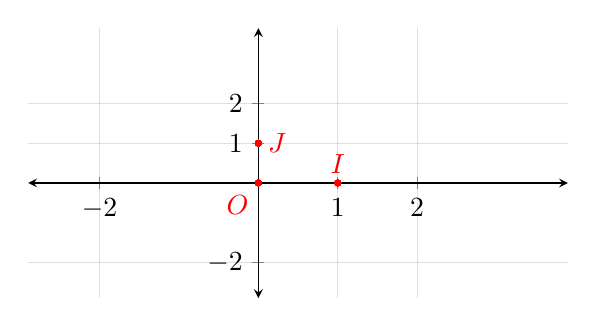
\begin{tikzpicture}[>=stealth, scale=1]
		\begin{axis}[xmin = -2.9, xmax=3.9, xtick={ -2,1,2}, ymin=-2.9, ymax=3.9, ytick={-2,1,2}, axis x line=middle, axis y 			line=middle, axis line style=<->, xlabel={}, ylabel={}, grid=both, grid style = {opacity=.5}, unit vector ratio=2 1]
		
			\addplot[red, mark=*, mark size = 1] (0,0) node[below=8pt, left] {$O$};
			\addplot[red, mark=*, mark size = 1] (1,0) node[above] {$I$};
			\addplot[red, mark=*, mark size = 1] (0,1) node[right] {$J$};
		\end{axis}
	\end{tikzpicture}
\end{center}
\end{ex}

\begin{defn}[Plan cartésien]
	Le plan cartésien est l'ensemble des couples $(x, y)$ de réels :
		\[ \bigset{ (x, y) \text{ tq. } x, y\in\R }. \]
\end{defn}

\begin{rmq}
Le plan cartésien est donc la combinaisons de \textbf{deux droites réelles}. 
Cette vision est conforme à la notion usuelle de \textit{dimension} : le plan carétsien est un ensemble à deux dimensions.
\end{rmq}

\begin{nomen}
On appelle un élément $(x;y)$ du plan un \textit{point} et $x, y$ ses \textit{coordonnées}.
\end{nomen}

\section{Opérations dans le plan}

\subsection{Distance entre deux points}

\begin{nota}
	Pour deux points $A$ et $B$ du plan, on note $AB$ la \textbf{distance} entre $A$ et $B$. \\
	La distance correspond au ``plus court chemin'' entre ces deux points. Une distance est donc un réel \textbf{positif}. \\
	Dans le plan cartésien, c'est simplement la longueur du segment [AB].
\end{nota}

\begin{rmq}
Attention, la distance mesurée ``physiquement'' (par exemple à l'aide d'une règle) n'est pas nécessairement égale à la distance ``mathématique'' entre deux points. En effet, les points $I$ et $J$ du repère ne sont pas toujours placés de façon à ce que les pas du repère soient égaux à 1 centimètre.
\end{rmq}

\begin{rapl}
Quelque soit $x \in \R, x^2 = (-x)^2$ (il s'agit d'une conséquence de la règle des signes vue au collège).
\end{rapl}

\begin{thm}[Distance]
	Soient $A(x_A, y_A)$, $B(x_B, y_B)$ deux points du plan dans un repère orthonormé.
	La distance $AB$ entre $A$ et $B$ est le nombre réel positif qui vérifie
		\[ AB^2 = (x_A - x_B)^2 + (y_A - y_B)^2 . \]
\end{thm}

\begin{proof}
On considère deux points $A$ et $B$ distincts dans un repère orthonormé. On place $B$ de tel façon que
\[ \left \{ \begin{array}{c c c } x_B & > & x_A \\ y_B & > & y_A \end{array} \right. \]
Les autres possibilités de placement conduisent à la même démonstration.

\begin{center}
	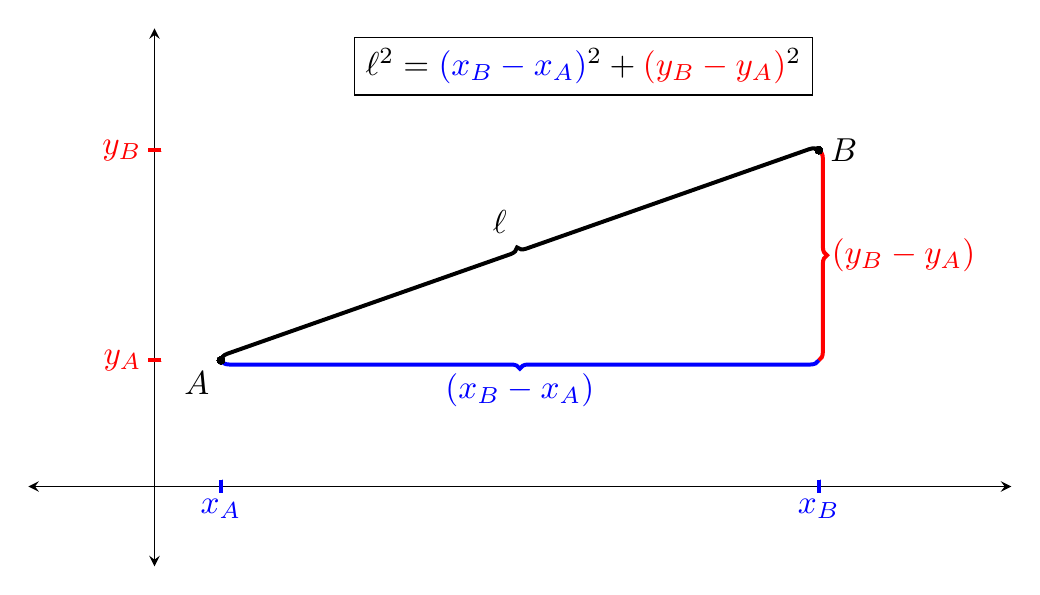
\begin{tikzpicture}[>=stealth, scale=1.2]
		\begin{axis}[xmin = -1.9, xmax=12.9, xticklabel=\empty, ymin=-1.9, ymax=10.9, yticklabel=\empty, axis x line=middle, axis y line=middle, axis line style=<->, xlabel={}, ylabel={}, ticks=none, clip=false, x=20pt]
		
			% A and B
			\addplot[black, mark=*, mark size = 1] (1,3) node[below left] {$A$};
			\addplot[black, mark=*, mark size = 1] (10,8) node[right] {$B$};
			
			
			\addplot[blue, mark=|, mark size = 2, very thick] (1,0) node[below] {$x_A$};
			\addplot[blue, mark=|, mark size = 2, very thick] (10,0) node[below] {$x_B$};
			\addplot[red, mark=-, mark size = 2, very thick] (0,3) node[left] {$y_A$};
			\addplot[red, mark=-, mark size = 2, very thick] (0,8) node[left] {$y_B$};
			
			% triangle
			\draw[red, very thick, decorate, decoration = {brace, mirror}] (axis cs:10,3) -- (axis cs:10,8) node [midway, right]{$(y_B - y_A)$};
			\draw[black, very thick, decorate, decoration = {brace}] (axis cs:1, 3) -- (axis cs:10,8) node [midway, above=10pt, left]{$\ell$};
			\draw[blue, very thick, decorate, decoration = {brace, mirror}] (axis cs:1, 3) -- (axis cs:10,3) node [midway, below]{$(x_B-x_A)$};
			
			% formula
			\addplot[black] (3,10) node[right, draw] {$\ell^2 = {\color{blue}(x_B-x_A)}^2 + {\color{red}(y_B - y_A)}^2$};
			
		\end{axis}
	\end{tikzpicture}
\end{center}

Les points $A$ et $B$ présentent un ``écart'' selon les deux dimensions du plan. 
En particulier, comme le plan est normé, on peut donc lire ces ``écarts'' directement via les coordonnées. 
Par exemple, l'écart horizontal entre $A$ et $B$ est donné par $x_B - x_A$.
De plus, comme le repère est orthogonal, on peut appliquer le théorème de Pythagore pour calculer la distance $AB$
\[ AB^2 = (x_A - x_B)^2 + (y_A - y_B)^2, \]
ce qui est la formule attendue.
\end{proof}

\begin{rmq}
Il faut ensuite calculer la racine carrée de $(x_A - x_B)^2 + (y_A - y_B)^2$ pour connaître la distance $AB$.
\end{rmq}

\subsection{Segment et milieu}

\begin{defn}[Segment]
Soit $A(x_A, y_A)$ et $B(x_B, y_B)$ deux points du plan cartésien. Le segment [AB] est l'ensemble des points de coordonnées :
\[ \{ (\lambda x_a + (1-\lambda) x_b , \lambda y_a + (1-\lambda) y_b) \text{ tels que } 0 \leq \lambda \leq 1 \} \] 
\end{defn}

\begin{rmq}
On peut voir les coordonnées des points du segment $[AB]$ comme les moyennes pondérées des coordonnées des points $A$ et $B$.
\end{rmq}

\begin{thm}[Coordonnées du milieu]
Soient $A$ et $B$ deux points du plan.
Alors le milieu $M$ du segment $[AB]$ a pour coordonnées :
	\[ M(x_M, y_M) \qquad \text{avec~~} \left \{ \begin{array}{c c c} x_M & = & \dfrac{x_A + x_B}2 \\ y_M & = & \dfrac{y_A + y_B}2 \end{array} \right. \]
\end{thm}

\begin{tikzpicture}[>=stealth, scale=1.2]
		\begin{axis}[xmin = -6.9, xmax=22.9, xticklabel=\empty, ymin=-2.9, ymax=4.9, yticklabel=\empty, axis x line=middle, axis y line=middle, axis line style=<->, xlabel={}, ylabel={},  ticks=none, clip=false, x=10pt]
		
			% A and B
			\addplot[black, mark=*, mark size = 1] (1,3) node[above right] {$A({\color{blue}x_A}; {\color{red}y_A})$};
			\addplot[black, mark=*, mark size = 1] (20,-2) node[below right] {$B({\color{blue}x_B}; {\color{red}y_B})$};
			
			
			\addplot[blue, very thick, mark=|, mark size = 2] (1,-.07) node[below] {$x_A$};
			\addplot[blue, very thick, mark=|, mark size = 2] (20,.07) node[above] {$x_B$};
			\addplot[red,very thick, mark=-, mark size = 2] (-.2,3) node[left] {$y_A$};
			\addplot[red, very thick, mark=-, mark size = 2] (-.2,-2) node[left] {$y_B$};
			
			% midpoint
			\addplot[black, mark=*, mark size = 1] (10.5,.5) node[above right] {$M$};	
			
			\addplot[blue, very thick, mark=|, mark size = 2] (10.5,-.07) node[below=3pt] {$\dfrac{x_A+x_B}2$};
			\draw[blue, dashed, very thick] (axis cs:10.5, 0) -- (axis cs:10.5,.5);
			
			\addplot[red, very thick, mark=-, mark size = 2] (-.2,.5) node[above=3pt, left] {$\dfrac{y_A+y_B}2$};
			\addplot[red, dashed, very thick, domain = 0:10.5, samples=2] {.5};			
			
			% dashed rectangle
			\draw[blue, dashed, very thick] (axis cs:1, 0) -- (axis cs:1,3);
			\draw[blue, dashed, very thick] (axis cs:20, 0) -- (axis cs:20,-2);
			\addplot[red, dashed, very thick, domain = 0:1, samples=2] {3};
			\addplot[red, dashed, very thick, domain = 0:20, samples=2] {-2};
			
			% formula
			%\addplot[black] (15,3) node[right, draw] {$M = \dfrac{A+B}2$};
			\addplot[black] (12,3) node[right, draw] {$M\Bigl({\color{blue}\dfrac{x_A+x_B}2} ; {\color{red}\dfrac{y_A+y_B}2}\Bigr)$};
			
			% [AB]
			
			\draw[-, black, dotted, thin] (axis cs:1,3) -- (axis cs:20,-2);
			
		\end{axis}
	\end{tikzpicture}

\begin{proof}
En prenant $\lambda = \frac12$ dans la définition du segment on vérifie que $M \in [AB]$. Il reste à vérifier que $M$ vérifie bien 
\[ AM = BM = \dfrac{AB}2 . \]
On effectue les calculs :
\begin{align*}
AM^2 & = (x_M - x_A)^2 + (y_M - y_A)^2 \\
& = \left (\dfrac{x_B - x_A}2 \right )^2 + \left (\dfrac{y_B - y_A}2 \right )^2 
\end{align*}
De même,
\begin{align*}
BM^2 & = (x_B - x_M)^2 + (y_B - y_M)^2 \\
& = \left (\dfrac{x_B - x_A}2 \right )^2 + \left (\dfrac{y_B - y_A}2 \right )^2 
\end{align*}
On remarque au passage que $\left (\dfrac{AB}2 \right )^2 = \dfrac14 AB  = AM^2 = AB^2$.
\end{proof}

\chapter{Fonctions}

Dans tout ce cours, on parlera de ``points de $\R$'' pour désigner des nombres réels. 
Cette expression est conforme à la représentation de l'ensemble des réels comme une droite (cf. chapitre 1).
Les nombres réels sont simplement des points de cette droite.

\section{Introduction}

\begin{defn}
On considère deux variables numériques (i.e. à valeurs dans $\R$) $x$ et $y$. On dit que la variable $y$ s'exprime \textbf{en fonction} de la variable $x$ si, à chaque valeur de $x$, on peut associer \textbf{une unique} valeur de $y$. On écrit alors $y(x)$ (ou parfois $y_x$) et on lit ``$y$ de x''. En d'autres termes, la valeur prise par la variable $y$ dépend de la valeur prise par la variable $x$.
\end{defn}

\begin{rmq}
Attention, à chaque valeur de $x$ correspond une unique valeur $y(x)$ de $y$. Pour autant, à plusieurs valeurs distinctes de $x$ peuvent être associées la même valeur de $y$. 
\end{rmq}

\begin{ex}
On considère une classe de 30 élèves. Chaque élève est représenté par sa position dans la liste d'appel (triée par ordre alphabétique). 
A chaque élève, on peut associer sa moyenne en Mathématiques. 
La variable ``Moyenne en mathématiques'' est donc fonction du numéro d'appel de chaque élève.
Pour autant, deux élèves distincts peuvent avoir la même moyenne en Mathématiques.
En revanche, un élève n'a qu'une seule moyenne en Mathématiques.
\end{ex}

\begin{defn}
Soient $x, y$ deux variables numériques. On définit la fonction $f$ qui à $x$ associe la valeur $y(x)$ par :
\[ \begin{array}{c c c c} 
f : & \R & \to & \R \\
& x & \mapsto & y(x)
\end{array} \]
et on note $y(x) = f(x)$. 
\end{defn}

\begin{nomen}
La lettre $f$ désigne une fonction, c'est-à-dire un objet qui transforme une quantité (par exemple $x$) en une autre quantité (par exemple $y$). Une fonction \textbf{n'est pas un nombre} ! En revanche, une fonction prend des valeurs numériques en certains points. Ainsi, $f(x)$ désigne la valeur prise par la fonction $f$ au point $x \in \R$ et $f(x)$ est un nombre réel.
\end{nomen}

\begin{rmq}
Le plus souvent, lorsque la fonction est nommée (par exemple $f$), on utilisera la notation $f(x)$ pour désigner la valeur prise par la variable $y$ au point $x$.
\end{rmq}

\begin{defn}[Domaine de définition]
	Soit $f$ une fonction numérique, 
	on note $\Dom_f \subset \R$ le domaine (ou ensemble) de définition de la fonction $f$.
	Le domaine de définition de $f$ correspond à l'ensemble des points de $R$ pour lesquels $f$ est bien définie
	(i.e. les points de $\R$ pour lesquels on peut calculer $f(x)$).
\end{defn}

\begin{ex}
La fonction de l'exemple précédent est définie uniquement sur les nombres entiers de 1 à 30. 
Si on la note $f$, on a alors 
\[ \Dom_f = \{ n \in \N \tq 1 \leq n \leq 30 \}. \]
\end{ex}

\begin{defn}[Image, antécédent]
Soit $f$ une fonction numérique,
\begin{itemize}
\item Soit $x \in \Dom_f$, on appelle \textbf{image} du point $x$ \textbf{par la fonction $f$} le réel $f(x)$.
\item Soit $y \in \R$, on appelle \textbf{antécédents} du point $y$ \textbf{par la fonction $f$} 
les éventuels points $x \in \Dom_f$ tels que $y=f(x)$.
\end{itemize}
L'image par $f$ d'un point de l'ensemble de définition est toujours unique. 
En revanche, l'antécédent d'un nombre réel par $f$ peut ne pas être unique ou même ne pas exister.
\end{defn}

\begin{ex}
On considère la fonction ``au carré'', que l'on nomme $g$ et que l'on définit comme ci-dessous :
\[ \begin{array}{c c c c}
	g : & \R & \to & \R \\
	& x & \mapsto & g(x)=x^2
\end{array} \]
L'image de -1 par la fonction $g$ est $g(-1)=1$. Le nombre 4 ademet deux antécédents par $g$, à savoir les réels $-2$ et $2$.
Le nombre 0 admet un unique antécdent par $f$ : 0. Enfin, le réel $-2$ n'admet pas d'antécédent par la fonction $f$.
\end{ex}

\begin{defn}[Forme algébrique]
On appelle forme algébrique d'une fonction $f$ une expression de $f(x)$ contenant des opérations mathématiques connues 
(addition, multiplication, etc.) ainsi que des constantes. \\
La forme algébrique d'une fonction permet de calculer explicitement l'image par $f$ des points de l'ensemble de définition de $f$.
\end{defn}

\begin{ex}
La forme algébrique de la fonction ``au carré'' est $f(x)=x^2$.
\end{ex}

\section{Intervalles de $\R$}

\begin{nota}
	On définit les signes suivants correspondant à des inégalités \textbf{strictes} et \textbf{larges}.
	\begin{multicols}{2}
	\begin{enumerate}[leftmargin=50pt]
		\item[$<$ :] strictement inférieur à
		\item[$\leq$ :] inférieur ou égal à
		\item[$>$ :] strictement supérieur à
		\item[$\geq$ :] supérieur ou égal à
	\end{enumerate}
	\end{multicols}
	On attire l'attention sur le fait que le « ou » est inclusif : $x \leq x$ est toujours vrai. 
\end{nota}

\begin{defn}[Intervalle borné]
	Un \textbf{intervalle} borné est un segment de la droite réelle $\R$. C'est donc un ensemble de nombres.
	Il est donné par une \textbf{borne inférieure} $a \in \R$ et une \textbf{borne supérieure} $b\in\R$ et peut contenir ou non ses bornes.
	
	\begin{enumerate}
		\item Si $a$ et $b$ sont contenues dans l'intervalle, on le note $[a ; b]$.
		\item Si $a$  est contenue dans l'intervalle mais $b$ ne l'est pas, on le note $[a ; b [$.
		\item Si $a$ n'est pas contenue dans l'intervalle mais $b$ l'est, on le note $] a ; b]$.
		\item Si ni $a$ ni $b$ ne sont contenues dans l'intervalle, on le note $] a ; b [$.
	\end{enumerate}
\end{defn}

\begin{ex}
Les intervalles suivants sont bornés.
	\begin{multicols}{2}
	\begin{enumerate}[label=$\bullet$]
		\item $[-1 ; 1]$
		\item $[-3 ; 1[$
		\item $\left]-10{,}341 ; \pi\right]$
		\item $\left]\sqrt{2} ; 130\right[$
	\end{enumerate}
	\end{multicols}
\end{ex}

\begin{prop}
Soient $a,b$ deux nombres réels tels que $a<b$. On a l'équivalence suivante :
\[ x \in ]a,b[ \equi a < x < b. \]
\end{prop}

\begin{ex}
$2 \in ]0,3[$, en revanche $3 \not \in ]0,3[$.
\end{ex}  

\begin{defn}[Intervalle non borné]
	Un intervalle n'est pas borné lorsque \textbf{au moins l'une} de ses deux bornes n'est pas fini.
	La borne inférieure peut être égale à $-\infty$ et la borne supérieure peut être égale à $\infty$.
	Comme l'infini n'est pas un nombre, un intervalle non borné est forcément ouvert à droite ou à gauche.
\end{defn}

\begin{ex}
	Les intervalles suivants ne sont pas bornés.
	\begin{multicols}{2}
	\begin{enumerate}[label=$\bullet$]
		\item $]-\infty; 2]$
		\item $]-\infty ; 3[$
		\item $]0; \infty[$
		\item $[-7, \infty[$
		\item $\R=]-\infty;\infty[$.
	\end{enumerate}
	\end{multicols}
\end{ex}

\begin{rmq}
On écrit toujours un intervalle de gauche à droite (en écrivant donc \textbf{la borne inférieure à gauche}). 
Un réel $x$ appartient à l'intervalle $[a,b]$ si, et seulement si, $a\leq x \leq b$. Lorsque l'intervalle est ouvert d'un côté, alors l'inégalité large devient strcite, par exemple $x \in ]0,1] \equi 0<x\leq1$.
\end{rmq}
	
\section{Représentation graphique}

Une fonction numérique prend ses valeurs sur la droite réelle et renvoie des valeurs sur la droite réelle.
Ainsi, il parait logique qu'une fonction numérique soit représenté comme un objet en deux dimensions, 
c'est-à-dire un objet du plan cartésien.
Il est heureux que nous ayons étudié le paln cartésien au chapitre précédent !

\begin{defn}[Courbe représentative]
Soit $f$ une fonction dont le domaine de définition est $\Dom_f$. 
On note $C_f$ la courbe représentative de $f$, $C_f$ est l'ensemble des points :
\[ C_f = \{ (x, f(x) \tq x \in \Dom_f \}. \]
$C_f$ est un sous-ensemble du plan cartésien.
\end{defn}

\begin{rmq}
	Connaître une fonction $f$ sur son domaine $\Dom_f$ c'est connaître sa courbe représentative $\C_f$, et vice versa.
	Cependant, il n'est pas toujours possible de dessiner $\C_f$ si le domaine $\Dom_f$ n'est pas borné, ou si $f$ prend des valeurs toujours plus grandes.
\end{rmq}

\begin{ex}
Ci-dessous \textbf{une partie} de la courbe représentative de la fonction f définie par :
\[ \begin{array}{c c c c}
f : & \R & \to & \R \\
& x & \mapsto & 2x+1
\end{array} \]

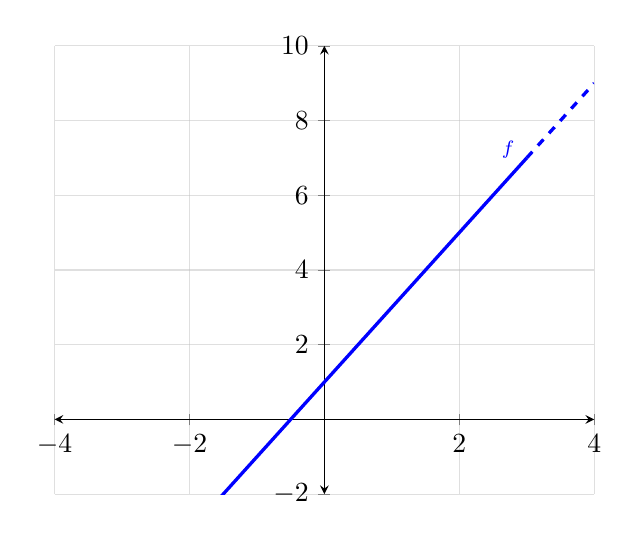
\begin{tikzpicture}[>=stealth, scale=1]
	\begin{axis}[xmin = -4, xmax=4, ymin=-2, ymax=10, axis x line=middle, axis y line=middle, axis line style=<->, xlabel={}, ylabel={}, 		grid=both, grid style = {opacity=.5}]]

	\addplot[blue, very thick, domain =-3:3, samples=2] {2*x+1}  node[above=3pt, left] {$\C_f$};
	\addplot[blue, very thick, dashed, domain =-4:-3, samples=2] {2*x+1} ;
	\addplot[blue, very thick, dashed, domain =3:4, samples=2] {2*x+1};

\end{axis}
\end{tikzpicture}
\end{ex}

\begin{rmq}
Les points du domaine de définition de $f$ sont placés \textbf{en abscisse}. 
Les images de ses points (les valeurs $f(x)$) sont placées \textbf{en ordonnée}. 
Autrement dit, la ``hauteur'' relative de la courbe représentative d'une fonction 
donne la grandeur relative des images des points de son domaine.
\end{rmq}

\begin{prop}
Soit $(x,y)$ un point du plan cartésien. On a l'équivalence suivante :
\[ (x,y) \in \C_f \equi y=f(x) . \]
En d'autres termes, un point $(x,y)$ quelconque du plan cartésien appartient à la courbe représentative de la fonction $f$
si, et seulement si, $x$ appartient au domaine de définition de $f$ et son image par $f$ est égale à $y$.
\end{prop}

\begin{ex}
Le point $(2,2)$ n'appartient pas à la courbe représentative de la fonction $f$ de l'exemple précédent. 
On a bien $2 \in \Dom_f$, cependant $f(2)=5 \neq 2$.
\end{ex}

\chapter{Evolution chiffrée}

\section{Population et sous-population}

\begin{defn}
On appelle population un ensemble d'individus et sous-population un sous-ensemble de ces individus.
\end{defn}

\begin{ex}
La sous-population des habitants d'Yzeure est un sous-ensemble de la population française.
Si on note $F$ la population française et $Y$ la population de la commune d'Yzeure, on a :
\[ Y \subset F \]
\end{ex}

\begin{defn}[Cardinal]
On appelle cardinal d'un ensemble fini le nombre d'éléments constituant cet ensemble. 
Pour un ensemble $E$ fini, on note $\abs{E}$ son cardinal.
\end{defn}

\begin{ex}
Le cardinal de la sous-population des habitants d'Yzeure est égal à 12 670 (au recensement de 2012).
\end{ex}

\begin{rmq}
Le cardinal d'un ensemble est un nombre \textbf{positif}.
\end{rmq}

\begin{prop}
On considère deux ensembles finis $E$ et $F$ tels que $F \subset E$. On a alors :
\[ \abs{F} \leq \abs{E} . \]
\end{prop}

\begin{defn}[Propotion d'une sous-population]
On considère une population $E$ et une sous-population $F$ ($F \subset E$).
La proportion d'individus de $E$ appartenant à $F$ est donnée par
\[ p = \dfrac{\abs{F}}{\abs{E}}. \]
Lorsque cette proportion est exprimée sous la forme d'une fraction de $100$, on parle alors de \textbf{pourcentage} d'éléments de $E$ appartenant à $F$.
\end{defn}

\begin{ex}
La proportion de Français résidant à Yzeure est égale à 
\[ p \approx \dfrac{12~670}{68 \times 10^6} \approx 1,86 \times 10^{-4} . \] 
Environ $0,0186 \%$ de la population française réside à Yzeure. 
\end{ex}

\begin{prop}
Pour $F \subseteq E$, on a :
\[ p \in [0;1] . \]
Autrement dit, la proportion d'individus d'une population appartenant à une sous-population donnée est un nombre compris entre 0 et 1,
ou encore le pourcentage d'individus appartenant à une sous-population est compris entre $0 \%$ et $100 \%$.
\end{prop}

\begin{proof}
Comme $F \subseteq E$, on a $0 \leq \abs{F} \leq \abs{E}$, d'où le résultat.
\end{rmq}

\begin{rmq}
Pour convertir une proportion $p$ en un pourcentage, il suffit de la multiplier par 100. 
Par exemple, si $p=\frac13$, alors $p \approx 33 \%$. 
On prendra garde au fait que de ne conserver qu'une partie des décimales du développement décimal d'une proportion 
revient à approximer cette dernière.
\end{rmq}

\begin{prop}[Sous-populations imbriquées]
On considère une popuation $E$ et deux sous-populations $F$ et $G$ telles que :
\[ G \subseteq F \subseteq E . \]
On note par ailleurs $p_F = \dfrac{\abs{F}}{\abs{E}}$ et $p_{G/F} = \dfrac{\abs{G}}{\abs{F}}$. On a alors 
\[p_{G} = p_F \times p_{G/F} . \]
Autrement dit, la proportion d'individus de $G$ dans la population totale est égale à la proportion d'individus de $F$ dans la population totale multipliée par la proportion d'individus de $G$ dans la sous-population $F$. 
\end{prop}

\begin{ex}
Dans un lycée, tous les élèves de seconde avec l'option Chinois sont regroupés dans une même classe.
Cette classe compte pour $3 \%$ de l'effectif total du lycée. 
Par ailleurs $20 \%$ des élèves de cette classe ont l'option Chinois.
Ainsi, le pourcentage de secondes ayant l'option Chinois dans le lycée est égal à :
\[ \frac3{100} \times \frac{20}{100} = 0,6 \% . \]
\end{ex}

\section{Evolution}

\begin{defn}[Augmentation, diminution]
Soit $x$ une quantité quelconque et $p \geq 0$ une proportion.
Une \textbf{augmentation} de $x$ d'une proportion $p \geq 0$ correspond à la somme
\[ x + x\cdot p = x \cdot (1+p).\]
Une \textbf{diminution} de $x$ d'une proportion $0\leq p \leq 1$ correspond à la différence
\[ x - x\cdot p = x \cdot (1-p).\]
\end{defn}

\begin{rmq}
On peut généraliser ces formules à une proportion $p$ négative. On a alors une seule formule :
\[ x + x\cdot p = x \cdot (1+p) , \]
et si $p<0$ alors l'évolution correspond à une diminution de $x$ d'une proportion $p$.
\end{rmq}

\begin{prop}[Evolution en pourcentage]
Soit $x$ une quantité quelconque et $p \%$ un pourcentage. Une augmentation de $p \%$ de $x$ correspond à l'opération :
\[ x \cdot \left (1 + \dfrac{p \%}{100} \right ) . \]
Inversement, une diminution de $p \%$ de $x$ correspond à l'opération :
\[ x \cdot \left (1 - \dfrac{p \%}{100} \right) . \]
\end{prop}

\begin{ex}
Un commerçant diminue le prix d'un article de $15 \%$. En notant $x$ le prix de l'article \textbf{avant diminution}, 
le prix après diminution correspond à $x \cdot \left ( 1 - \frac{15}{100} \right ) = x \cdot 0,85$.
\end{ex}

\begin{prop}[Astuce de calcul]
Soient $A$ et $B$ deux nombres réels positifs ou nuls.
Les quantités \og $A\%$ de $B$ \fg ~et \og $B\%$ de $A$ \fg ~sont égales.
\end{prop}

\begin{rmq}
Cette proposition permet de calculer facilement certaines proportion. 
Par exemple, il est plus facile de calculer $20 \%$ de 45 que $45 \%$ de 20.
\end{rmq}

\begin{defn}[Variation absolue et relative]
On considère une quantité quelconque prenant les valeurs $x_1$ (valeur initiale) \textbf{puis} $x_2$ (valeur finale).
\begin{itemize}
\item
La variation absolue de cette quantité correspond à la différence $x_2 - x_1$.
\item 
La variation relative de cette quantité correspond au rapport  :
\[ \dfrac{x_2 - x_1}{x_1} \]
\end{itemize}
\end{defn}

\begin{ex}
Le prix au kilogramme de la farine de blé passe de 0,74 \euro~ à 0,82 \euro.
\begin{itemize}
\item
La variation absolue de ce prix est égale à 0,08 \euro soit 8 centimes.
\item 
La variation relative de cette quantité est égale à :
\[ \dfrac{0,82 - 0,74}{0,74} \approx 0,108 \] 
ce qui correspond à un augmentation d'environ $10,8 \%$.
\end{itemize}
\end{ex}

\begin{defn}[Coefficient multiplicateur]
On considère une quantité quelconque prenant les valeurs $x_1$ (valeur initiale) \textbf{puis} $x_2$ (valeur finale).
Le coefficient multiplicateur entre ces deux valeurs correspond au rapport :
\[ m = \dfrac{x_2}{x_1} . \]
\end{defn}

\begin{prop}
Soient $x_1$ et $x_2$ les valeurs successives d'une quantité et $m = \frac{x_2}{x_1}$ le coefficient multiplicateur correspondant.
On distingue trois cas.
\begin{enumerate}
    \item si $x_1=x_2$, alors $m=1$ ;
    \item si $x_1 < x_2$, alors $m>1$ ; 
    \item si $x_1 > x_2$, alors $m<1$.
\end{enumerate}
\end{prop}

\begin{rmq}
On peut convertir ce coefficient multiplicateur $m$ en une proportion en utilisant la formule :
\[ p = 1 - m \equi m = 1 + p . \]
En effet :
\begin{itemize}
\item si $m=1$, la quantité n'a pas évoluée et $p = 0$ ;
\item si $m>1$, la quantité a agumentée et $p>0$, ce qui correspond à une augmentation d'une proportion $p$ ;
\item si $m<1$, la quantité a diminuée et $p<0$, ce qui correspond à une diminution d'une proportion $-p$.
\end{itemize}
\end{rmq}

\begin{thm}[Evolutions successives]
On considère une grandeur quelconque subissant deux évolutions successives 
et on note $m_1$ et $m_2$ les facteurs multiplicatifs de ces deux évolutions.
Alors, le facteur mulitplicatif total est donné par 
\[ m=m_1 \times m_2 . \]
En d'autres termes, lors d'évolutions successives, les facteurs multiplicatifs sont multipliés entre eux. 

\begin{center}
	\resizebox{11cm}{!}{
	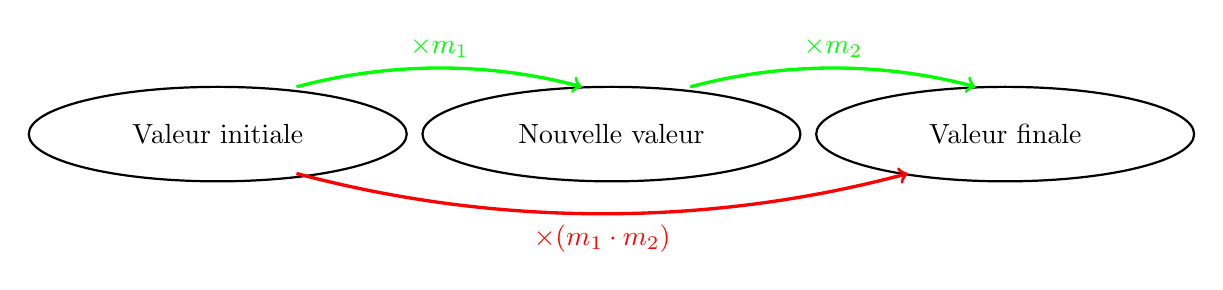
\begin{tikzpicture}
		% nodes
		\draw[thick] (0,0) ellipse (2.4cm and .6cm) node {Valeur initiale};
		
		\draw[thick] (5,0) ellipse (2.4cm and .6cm) node {Nouvelle valeur};
		
		\draw[thick] (10,0) ellipse (2.4cm and .6cm) node {Valeur finale};
		
		% vertices
		\draw[->, very thick, green] (1cm,.6cm) arc (105:75:7) node[midway, above] {$\times m_1$};
		\draw[->, very thick, green] (6cm,.6cm) arc (105:75:7) node[midway, above] {$\times m_2$};
		
		\draw[->, very thick, red] (1cm,-.5cm) arc (-105:-75:15) node[midway, below] {$\times (m_1\cdot m_2)$};
	\end{tikzpicture}
	}
\end{center}
\end{thm}

\begin{thm}[Evolutions réciproques]
On considère une grandeur quelconque subissant une évolution de coefficient multiplicateur $m$.
Alors le coefficient multiplicateur qui permet de revenir à la valeur initiale de cette grandeur correspond à :
\[ m' = \dfrac1{m} \]

	\begin{center}
	\resizebox{11cm}{!}{
	\begin{tikzpicture}
		% nodes
		\draw[thick] (0,0) ellipse (2.4cm and .6cm) node {Valeur initiale};
		
		\draw[thick] (5,0) ellipse (2.4cm and .6cm) node {Nouvelle valeur};
		
		\draw[thick] (10,0) ellipse (2.4cm and .6cm) node {Valeur initiale};
		
		% vertices
		\draw[->, very thick, green] (1cm,.6cm) arc (105:75:7) node[midway, above] {$\times m$};
		\draw[->, very thick, green] (6cm,.6cm) arc (105:75:7) node[midway, above] {$\times \dfrac{1}{m}$};
		
		\draw[->, very thick, red] (1cm,-.5cm) arc (-105:-75:15) node[midway, below] {$\times \left(m\cdot \dfrac{1}{m}\right) = \times 1$};
	\end{tikzpicture}
	}
	\end{center}
\end{thm}

\end{document}